\chapter{Experimental setup}
In this section, we will give an overview of the experimental setup of the Large Hadron Collider (LHC) and the Compact Muon Solenoid (CMS) experiment as it pertains to the~\ttH~search during Run II of the LHC. First, we will review the essential details of the LHC machine and the main experiments on the LHC ring. At the time of writing, the LHC, which is located at CERN nearby Geneva, is the highest-energy hadron collider in the world and the only experimental apparatus where Higgs bosons can be produced and studied directly. Next, we will discuss the CMS experiment, which is one of the two general-purpose detectors on the LHC ring. In particular, we will describe the subsystems and reconstruction algorithms of the detector that are crucial to the~$\ttH$~search.

\section{The Large Hadron Collider}
The LHC is a hadron collider situated in the 26.7-km tunnel of the Large Electron Positron (LEP) machine. The hadrons, either protons or heavy ions, are accelerated in several stages by the pre-accelerator complex of the LEP, shown on figure~\cref{fig:lhc_accelerators}. In the description that follows, we will consider only proton-proton collisions for concreteness. The protons are accelerated by the linear accelerator LINAC to 50~MeV, the proton synchrotron booster (PSB) to 1.4~GeV, the proton synchrotron (PS) to 26~GeV and by the super proton synchrotron to 450~GeV. The protons are injected in bunches of~$N_b \simeq 10^{11}$~protons per bunch into the main rings with a frequency of 40~MhZ, such that the nominal bunch spacing is 25~ns and there are~$n_b=\mathcal{O}(2500)$~bunches per beam.

\begin{figure}
\begin{centering}
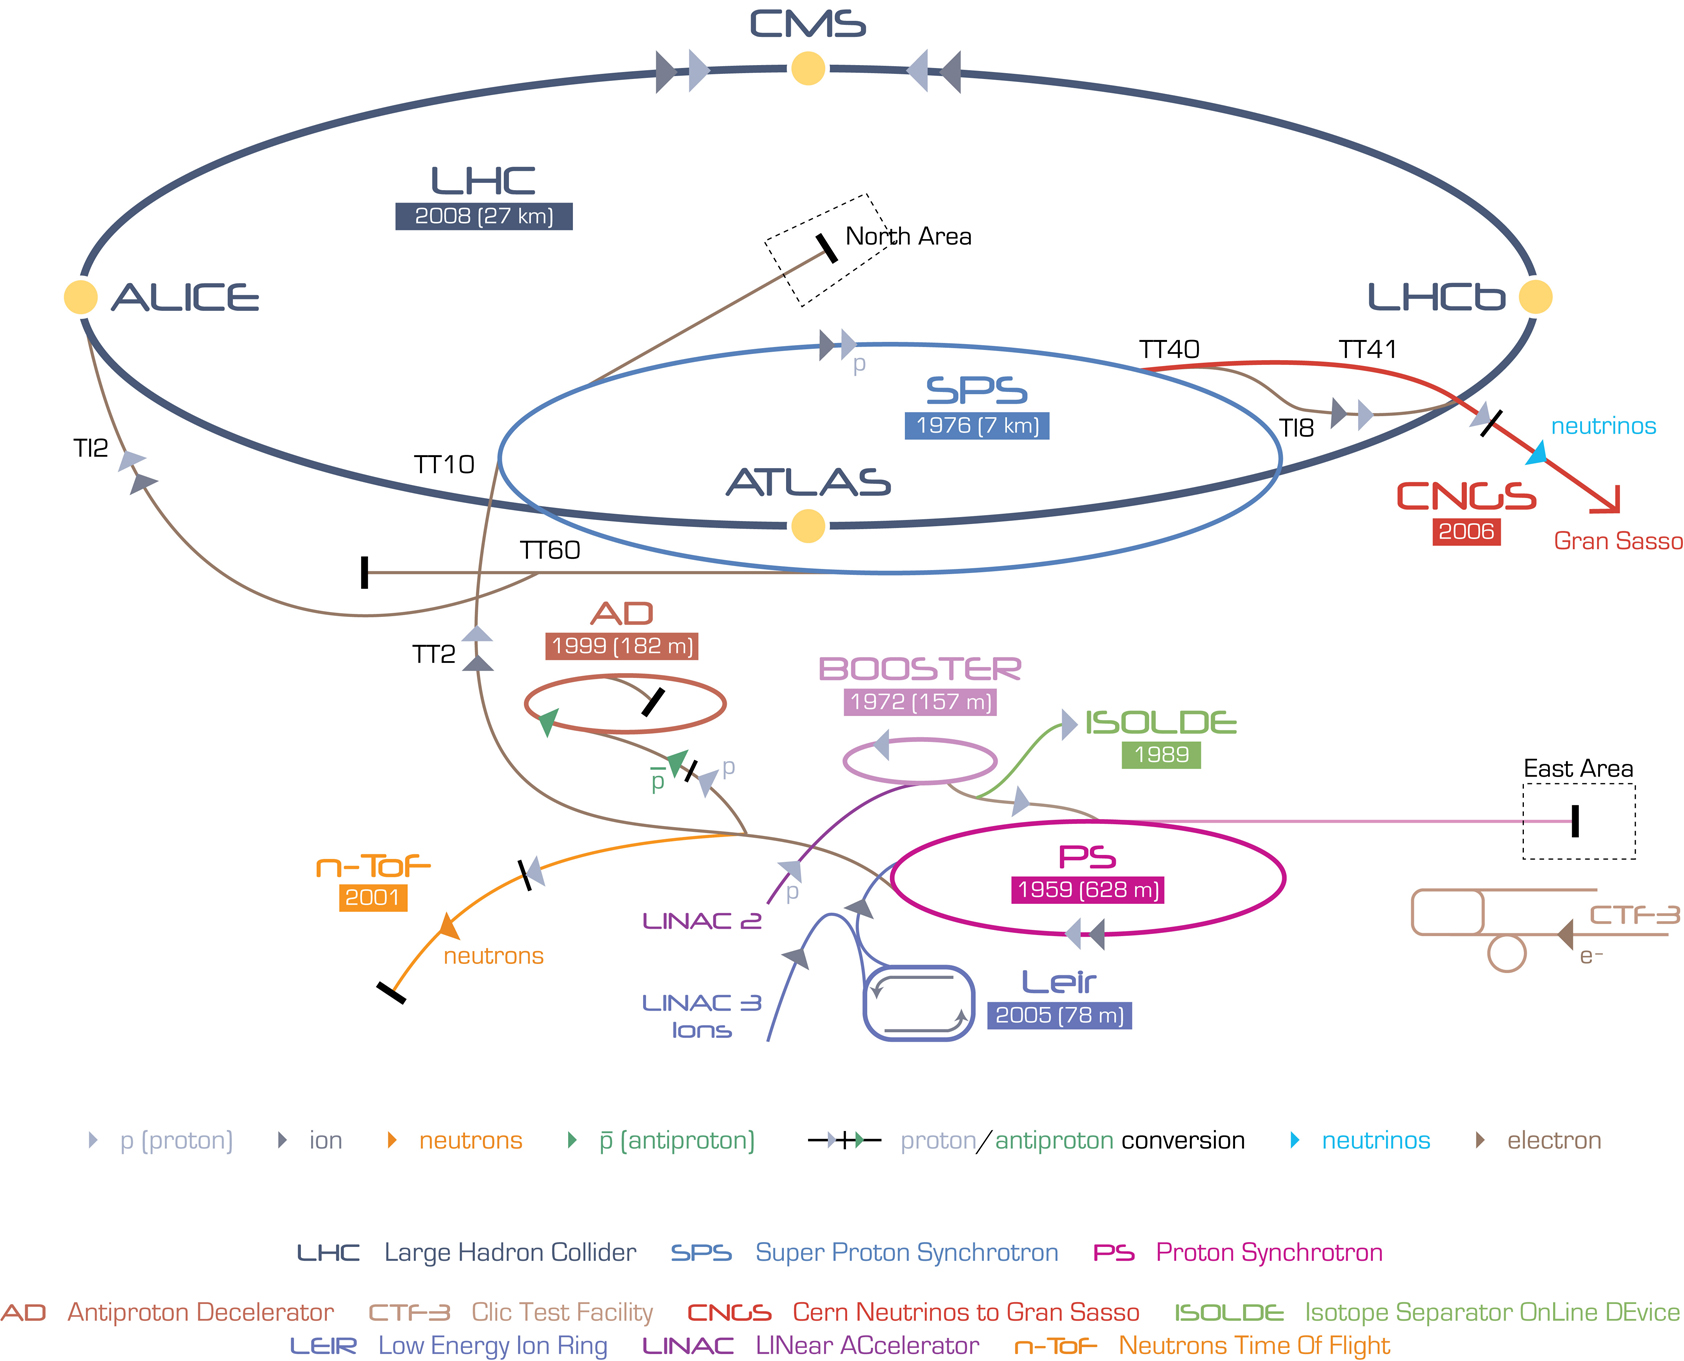
\includegraphics[width=0.8\textwidth]{figures/exp/accelerators.jpg}
\caption[The LHC accelerator complex]{The LHC accelerator complex, where the protons are accelerated by LINAC 2, the PS and the SPS before being injected into the main LHC ring, where they are collided in the 4 interaction points.}
\label{fig:lhc_accelerators}
\end{centering}
\end{figure}

\subsection{The accelerator complex}
In the main accelerator system consisting of two concentric counter-rotating rings, where superconducting magnets with a nominal B-field~$B=8.33~\mathrm{T}$~are used to bend and focus the beams, the protons are accelerated to the center-of-mass energy~$\sqrt{s} = 13$~TeV. Dipole magnets, depicted on~\cref{fig:lhc_magnet}, are used to bend the beam and multipole magnets for focusing. Both rings are located in beam pipes with an inner diameter of 48~mm within the same vacuum chamber in a so-called twin-bore design, dictated by the size of the tunnel. The magnets are kept at an operating temperature below 2K using liquid He-4. These proton bunches are collided at 4 interaction points and the beams can be sustained for up to 24~hours. The machine is characterized by the designed instantaneous luminosity of~$L=10^{34}~\mathrm{cm}^{-2}\mathrm{s}^{-1}$, which has been exceeded in 2017 by a factor of 1.58.

\begin{figure}
\begin{centering}
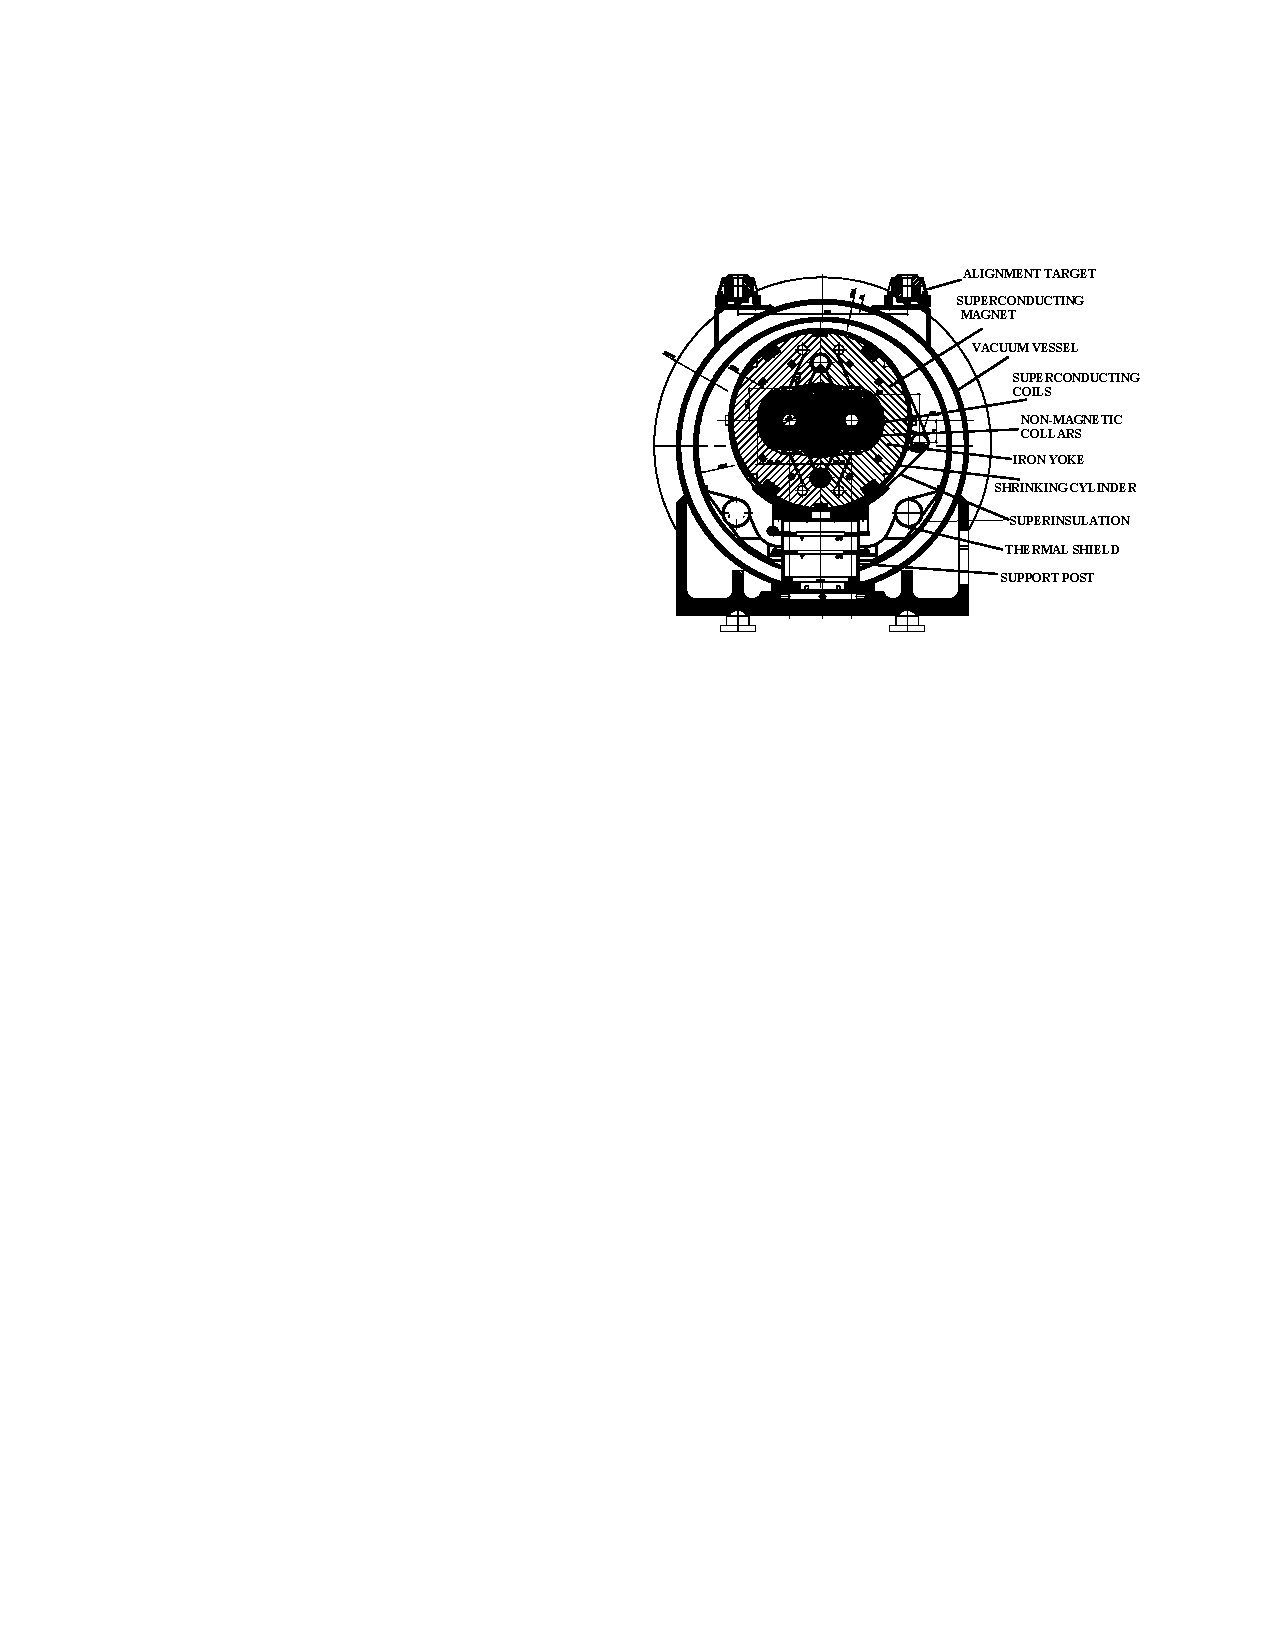
\includegraphics[width=0.8\textwidth]{figures/exp/cryodipole.pdf}
\caption{Cross-section of the LHC dipole magnet.}
\label{fig:lhc_magnet}
\end{centering}
\end{figure}

The proton-proton collisions at the LHC interaction points result in a number of events per second given by~$N_i = L \sigma_i$~for a process that has a cross-section~$\sigma_i$~at a given instantaneous luminosity~$L$. For the LHC, the machine luminosity is given by the Gaussian beam profile through

\begin{equation}
L = \frac{N_b^2 n_b f_\mathrm{rev} \gamma_r}{4 \pi \epsilon_n \beta^*} F
\end{equation}
where~$f_{\mathrm{rev}}$~is the number of revolutions per second and~$\gamma_r$~is the relativistic Lorentz factor. The beam is further described by the normalized transverse emittance~$\epsilon_n$~and the beta function~$\beta^*$~of the beam at the interaction point, which are related to the transverse beam size at a location~$s$~along the beam through~$\sigma(s) = \sqrt{\epsilon_n \beta(s)}$. The transverse emittance characterizes the spread of particles in the position-momentum phase space throughout their orbits. The beams cross at the interaction points at an angle~$\theta_c$, which results in luminosity reduction by a factor

\begin{equation}
F = \biggl[1 + \bigr( \frac{\theta_c \sigma_z}{2 \sigma^*} \bigr)^2 \biggr]^{-1/2}
\end{equation}
where~$\sigma_z$~is the bunch length and~$\sigma^*$~the transverse bunch size. The~$\beta^*$~parameter dictates the size of the beam at the interaction point, which is tuned to the luminosity requirements of the experiment and in turn limited by the aperture of the focusing magnets. The maximum beam size in the transverse direction is~$\sigma=1.2~\mathrm{mm}$, limited by the dimensions of the beam screen. The instantaneous luminosity decays over time during a physics run due to beam loss from the collisions, such that the luminosity decreases by~$1/e$~during approximately~$15\ h$.

The total number of collisions in a given unit of time is characterized by the integrated luminosity~$\mathcal{L} = \int L\ \mathrm{d}t$~and is limited to around~$80-120~\mathrm{fb}^{-1}$~per year under perfect conditions, assuming around 200 days of operation and on average 7 hours of turn-around time between runs for filling the beams and accelerating to data-taking energies.

During the 2016 data taking period considered in this thesis, the LHC operated at a center-of-mass energy of~$\sqrt{s} = 13~\mathrm{TeV}$,~$\beta^* = 40~\mathrm{cm}$~and delivered around~$\mathcal{L} = 40~\mathrm{fb}^{-1}$~of proton-proton data to the ATLAS and CMS experiments. With an inelastic pp cross-section of~$\sigma_{pp} \simeq 77$~mb~\cite{VanHaevermaet:2016gnh}, this correspond to about~$10^{15}$~pp interactions per year.

\subsection{Experiments at the LHC}
The collision data form the LHC is recorded by 2 general purpose detectors, CMS and ATLAS (A Toroidal LHC ApparatuS), and 2 experiments with a more specialized physics program, LHCb and ALICE (A Large Ion Collider Experiment), located at the 4 interaction points. Overall, the general properties and physics goals of the experiment are as follows.

\subsubsection{CMS}
The main characteristic of CMS is the superconducting solenoid, which provides a magnetic field of 3.8T that enables the momentum of charged particles to be measured with high accuracy. Inside the solenoid volume are silicon pixel and strip trackers, an electromagentic calorimeter (ECAL) comprised of~$\mathrm{PbWO}_4$~crystals and a brass-scintillator hadronic calorimeter (HCAL). Outside the solenoid volume is the steel return yoke for the magnetic field, which contains gas-ionization chambers used to measure muons. The CMS detector was designed to meet a dimuon, diphoton and dielectron mass resolution of~$1\%$~at 100~GeV~\cite{Chatrchyan:2008aa}.

\subsubsection{ATLAS}
The overall layout of the ATLAS machine differs from CMS mainly with respect to the configuration of the magnetic fields, where a central superconducting solenoid with B=2T houses the semiconductor trackers, with the lead-liquid argon (LAr) electromagnetic calorimeter and the hadronic calorimeters outside the solenoid volume. The muon systems are embedded in an outer air-core toroidal system that minimizes multiple scattering.

\subsubsection{LHCb}
The primary goal of the LHCb experiment is to study heavy flavour physics, in particular rare decays of beauty and charm hadrons and searching for indirect evidence for new physics in CP-violation, exploiting the large rate of B-meson production at the LHC. The LHCb detector is a single-arm spectrometer with a forward angular coverage of 10 to 250-300~mrad, featuring a beryllium beampipe that is highly transparent to particle fluxes and an accurate vertexing system. LHCb operates at an instantaneous luminosity that is two orders of magnitude lower than CMS and ATLAS in order to minimize multiple pp interactions per bunch crossing.

\subsubsection{ALICE}
The ALICE detector is designed to study heavy ions, focusing on QCD measurements, in particular the study of strongly interacting matter at the high temperatures and densities achievable in nucleon-nucleon collisions. It features general-purpose detectors in the barrel, embedded in a solenoid and muon spectrometers in the forward direction. The ALICE detector is specifically optimized to study global event observables such as particle multiplicity and energy flow. 

\subsubsection{Purpose}
Both the CMS and ATLAS experiments have the broad physics goal of discovering the Higgs boson, studying its properties and searching for any new resonances at high energies. The discovery of the Higgs boson was realized during Run I of the LHC, with both experiments reporting a significant excess in 2012 that is compatible with a SM Higgs boson~\cite{Aad:2012tfa,Chatrchyan:2012xdj}. In the following section, we will discuss the essential aspects of the CMS experiment in more detail.

\section{The CMS detector}
The coordinate system adopted by CMS is centered at the collision point, with the x-axis pointing inward towards the LHC ring, y-axis vertically upward and the z axis along the beamline towards east in the direction of the Jura mountains. The azimuthal angle~$\phi$~is measured from the x axis in the plane transverse to the beam. The polar angle is measured from the z-axis and it defines the pseudorapidity~$\eta = -\ln{\tan{\theta/2}}$. The CMS detector follows a layered design that encapsulates the interaction region completely in the azimuthal direction and provides good coverage in the polar direction. In order to achieve this, the detector is divided into a barrel component and two endcaps, as can be seen on~\cref{fig:cms_experiment}. A transverse slice of the experiment can be seen on~\cref{fig:cms_slice}, where the overall layout of the subdetectors is depicted along with example particle trajectories for muons, electrons, charged and neutral hadrons and photons. 

\begin{figure}
\begin{centering}
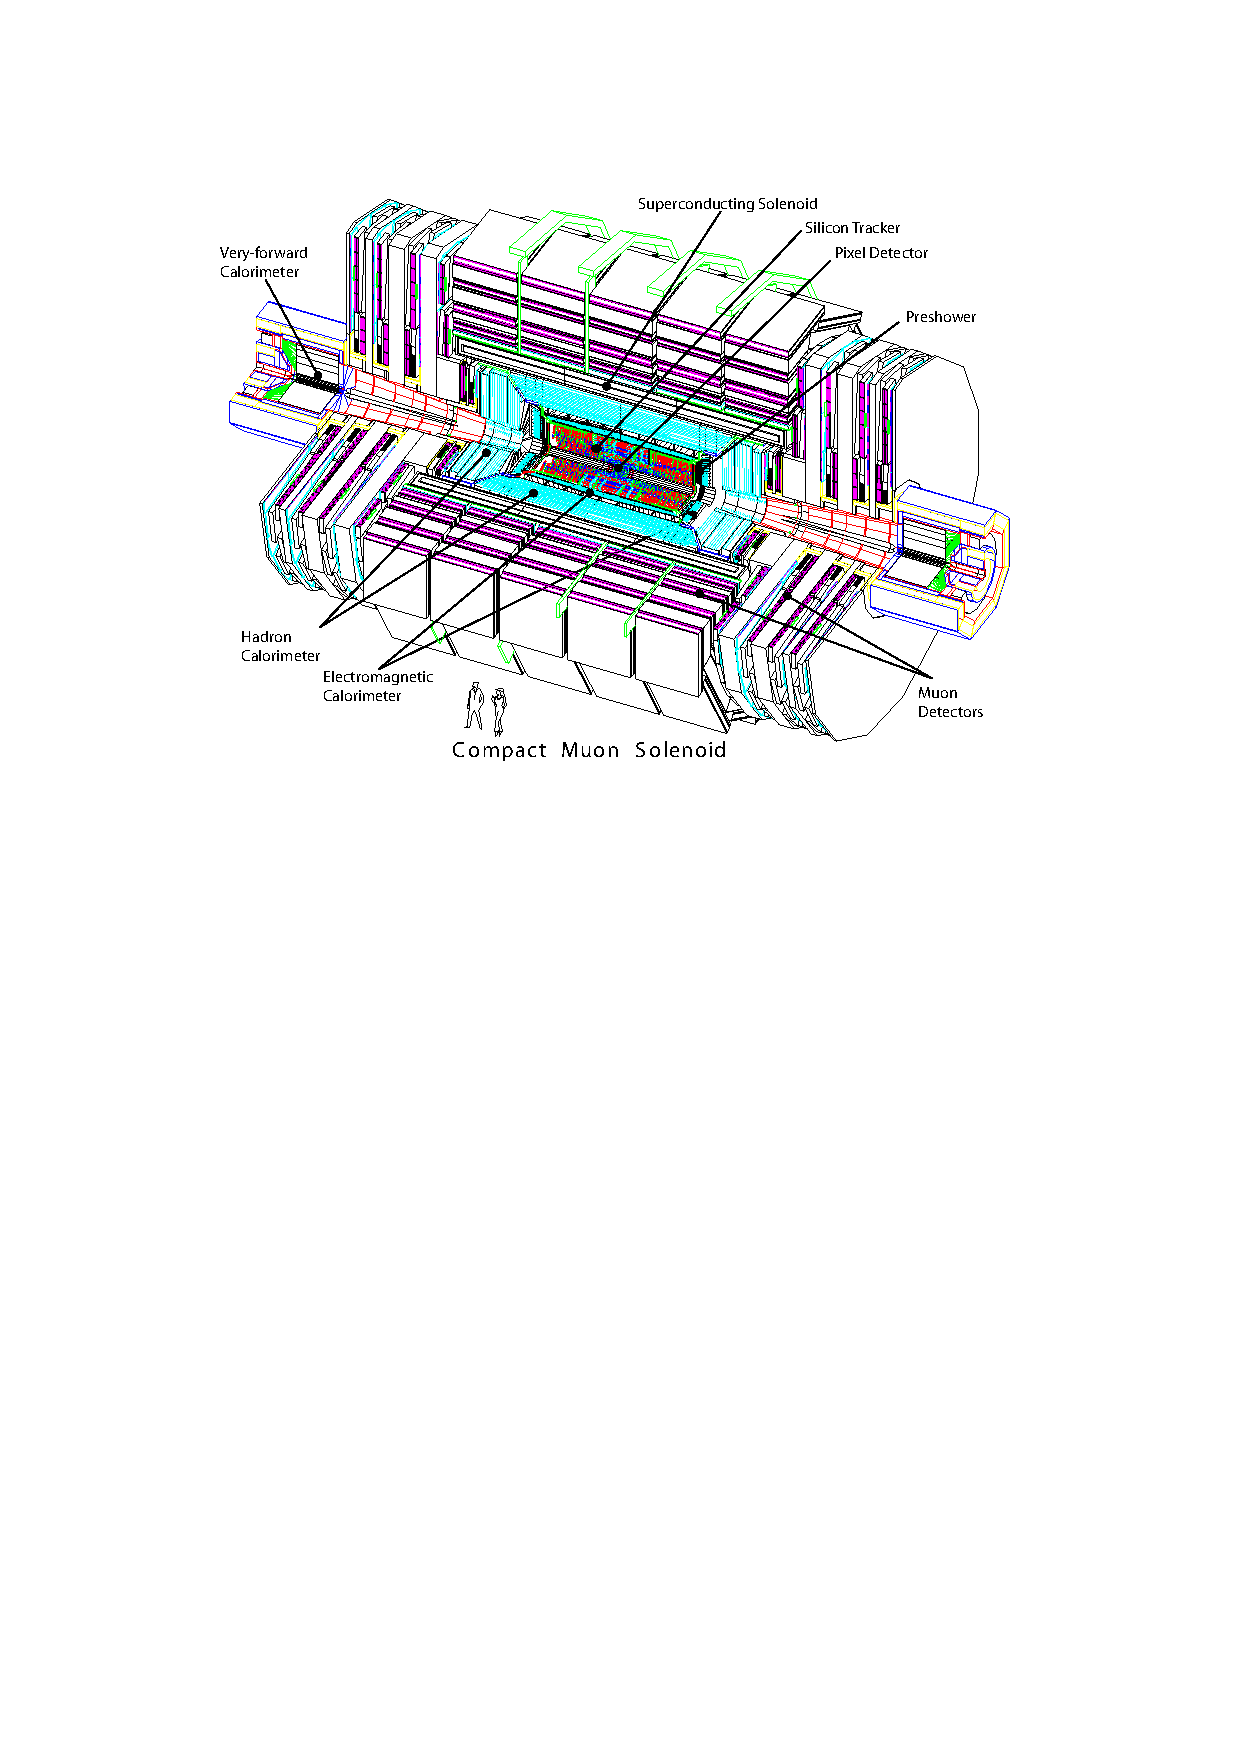
\includegraphics[width=0.8\textwidth]{figures/exp/cms.pdf}
\caption{The cross-section of the CMS experiment.}
\label{fig:cms_experiment}
\end{centering}
\end{figure}

\begin{figure}
\begin{centering}
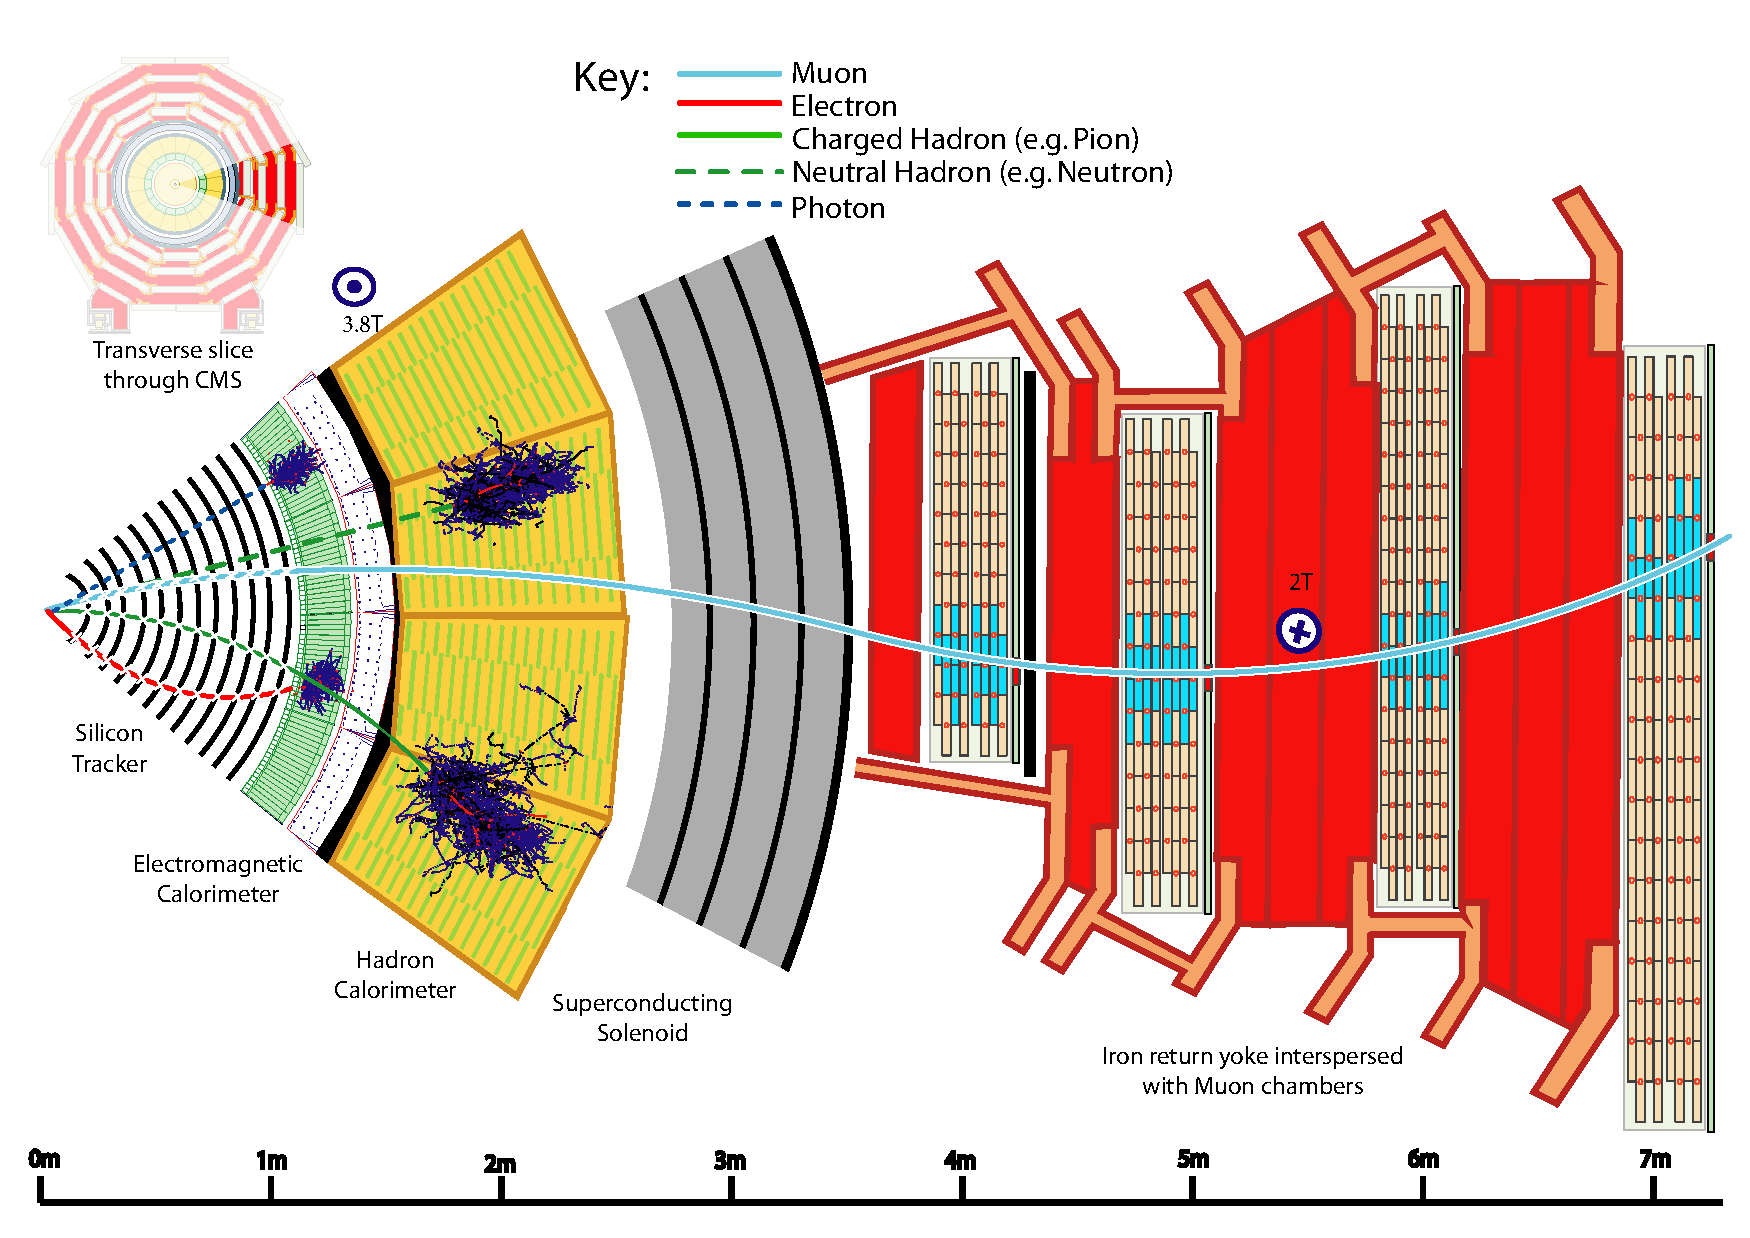
\includegraphics[width=0.8\textwidth]{figures/exp/cms_slice.pdf}
\caption{A view of a transverse slice of the CMS detector with the subsystems.}
\label{fig:cms_slice}
\end{centering}
\end{figure}

\subsection{The superconducting magnet}
The 3.8T magnetic field, which is essential for measuring the momenta and charge of charged particles, is created by the 220~ton superconducting solenoid, which has a diameter of 6~m and a length of 12.5~m. The energy stored in the relatively thin NbTi conductor reaches up to 2.6~GJ, therefore the mechanical deformations in the magnet during energizing can be significant. The iron return yoke of the magnetic field consists of sections which house the muon chambers and thus guarantee a sufficient field strength in the muon spectrometer region.

\subsection{Inner tracking system}
The inner tracking system measures the momenta and trajectories of charged particles from the primary vertex in the interaction point and any secondary vertices associated to the decay of long-lived particles such as b hadrons. The magnetic field is homogeneous within the tracker volume, which has a length of 5.8~m and a diameter of 2.5~m. The number of simultaneous inelastic collision (pileup) events per bunch crossing in pp collisions can be significant at the LHC, with nominal values around~$N_{PV} = 20-50$, but reaching an order of magnitude more in the HL-LHC. Therefore, the tracking system has to cope with high particle fluxes of up to~$10^3$~particles per bunch crossing every 25~ns and be able to associate signals to the correct bunch crossing.

\subsubsection{Pixel detector}
In order to keep the hit occupancy around 1\%, pixel detectors have to be used in the inner region of the tracker. The inner tracker consists of a 3-layer silicon pixel detector with layers at 4.4~cm, 7.3~cm and 10.2~cm and a silicon strip detector with 10 layers extending out to radii of 1.1~m. The pixels in the inner layer measure~$100\times150~\mathrm{\mu m}^2$~in the~$r-\phi$~and~$z$~directions, which is driven by the secondary vertex and impact parameter resolution necessary for the detection of heavy flavour states. The pixel detector covers the range range~$|\eta| < 2.5$~and consists of the barrel layers (BPix) and two endcap discs (FPix), located in such a way as to guarantee at least 3 pixel hits over almost the full range, as seen on~\cref{fig:cms_pixel}. By reading out the analog pulse height using charge sharing which results from the the B field, a hit resolution of 15-20~$\mathrm{\mu m}$~can be achieved. In total, the pixel detector covers an area of~$1~\mathrm{m}^2$~and consists of around 66 million pixels.

\begin{figure}
\begin{centering}
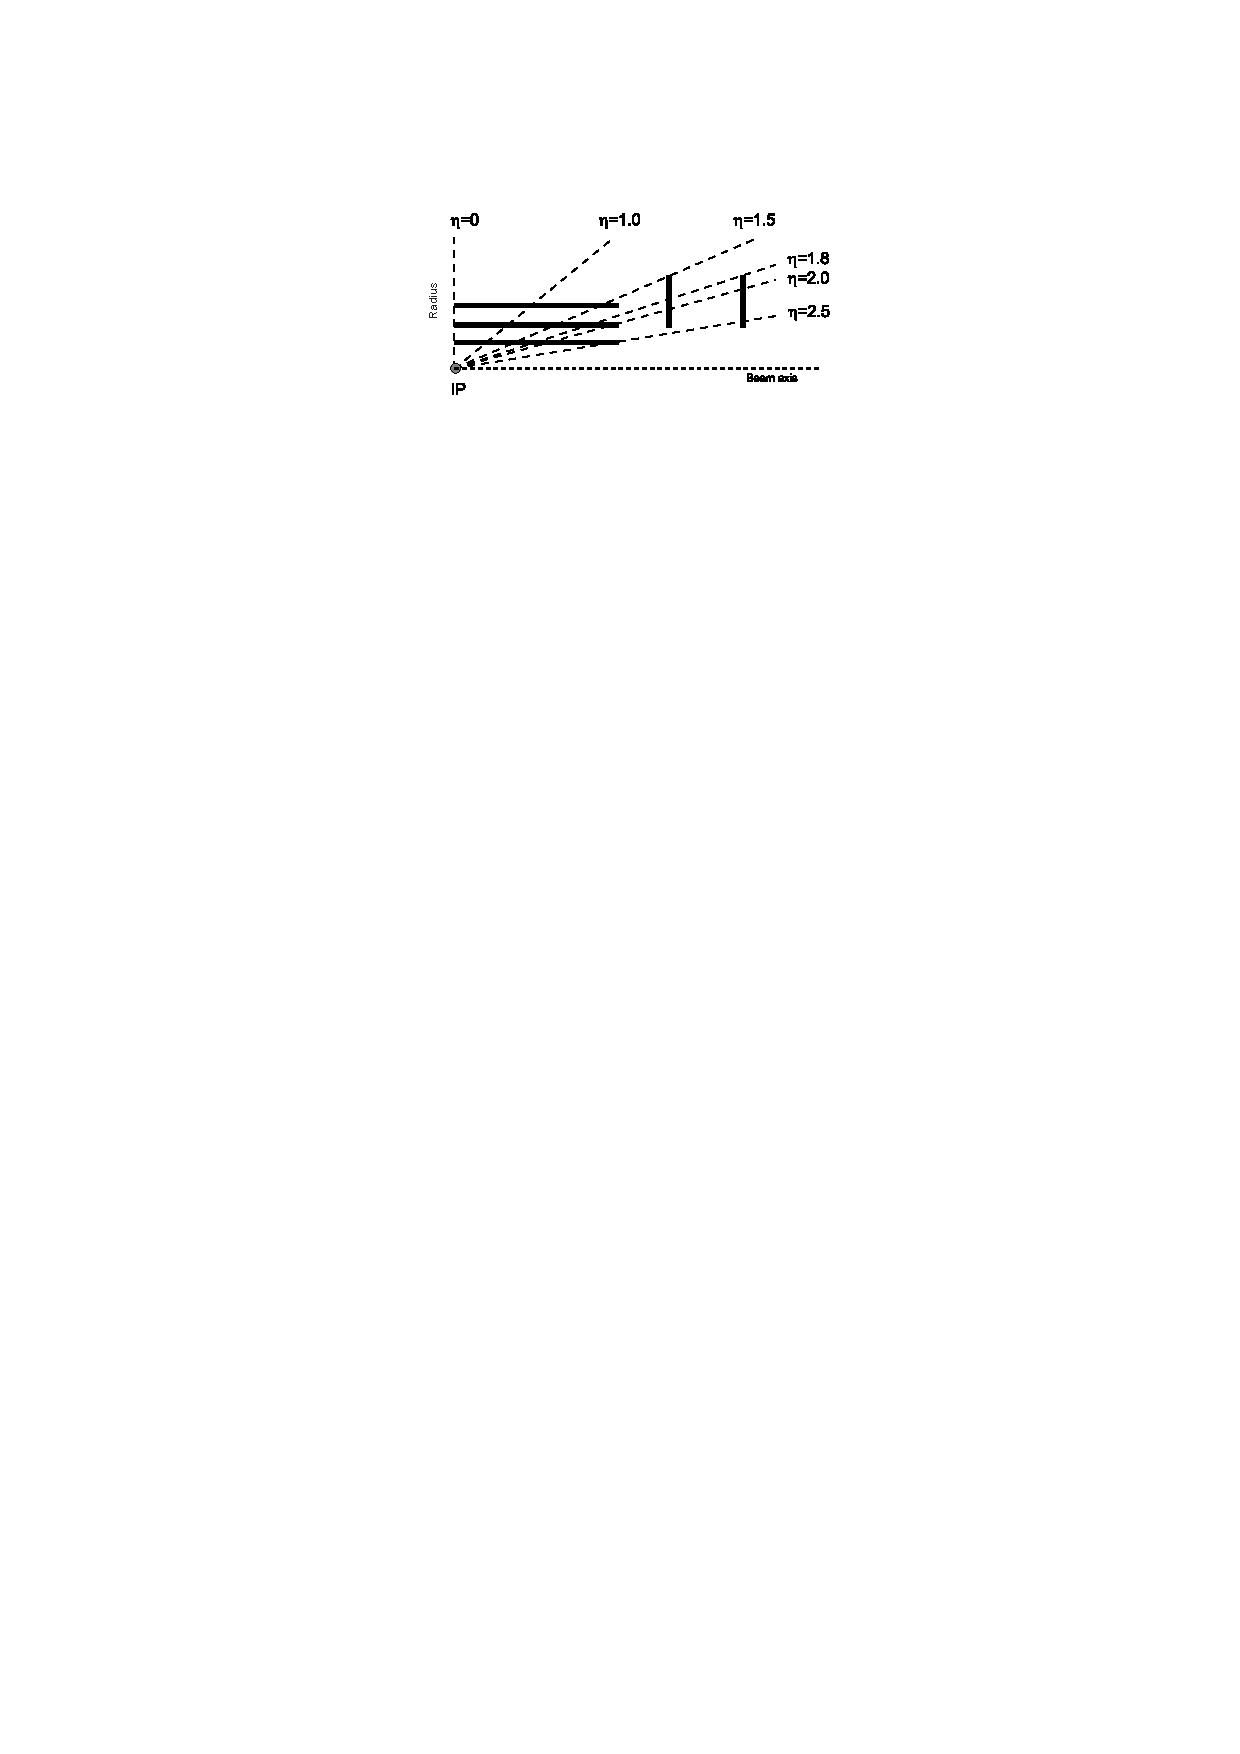
\includegraphics[width=0.6\textwidth]{figures/exp/pixel.pdf}
\caption{The schematic overview of the CMS pixel tracker.}
\label{fig:cms_pixel}
\end{centering}
\end{figure}

\subsubsection{Silicon strip tracker}
At larger radii, the occupancy decreases, such that silicon strips with a typical size of~$10\mathrm{cm} \times 80\mathrm{\mu m}$~are used in the silicon strip tracker. The tracker consists of several layered subsystems as shown on~\cref{fig:cms_tracker}, in particular, the tracker inner barrel and discs (TIB/TID), the outer barrel (TOB) and the tracker endcaps (TEC). The TIB/TID delivers 4 measurements of a track in the~$r-\phi$~direction, the TOB 6 measurements, and the TEC 9 measurements per particle trajectory. The strip pitch increases at larger radii to compensate for the reduction in particle flux.

\begin{figure}
\begin{centering}
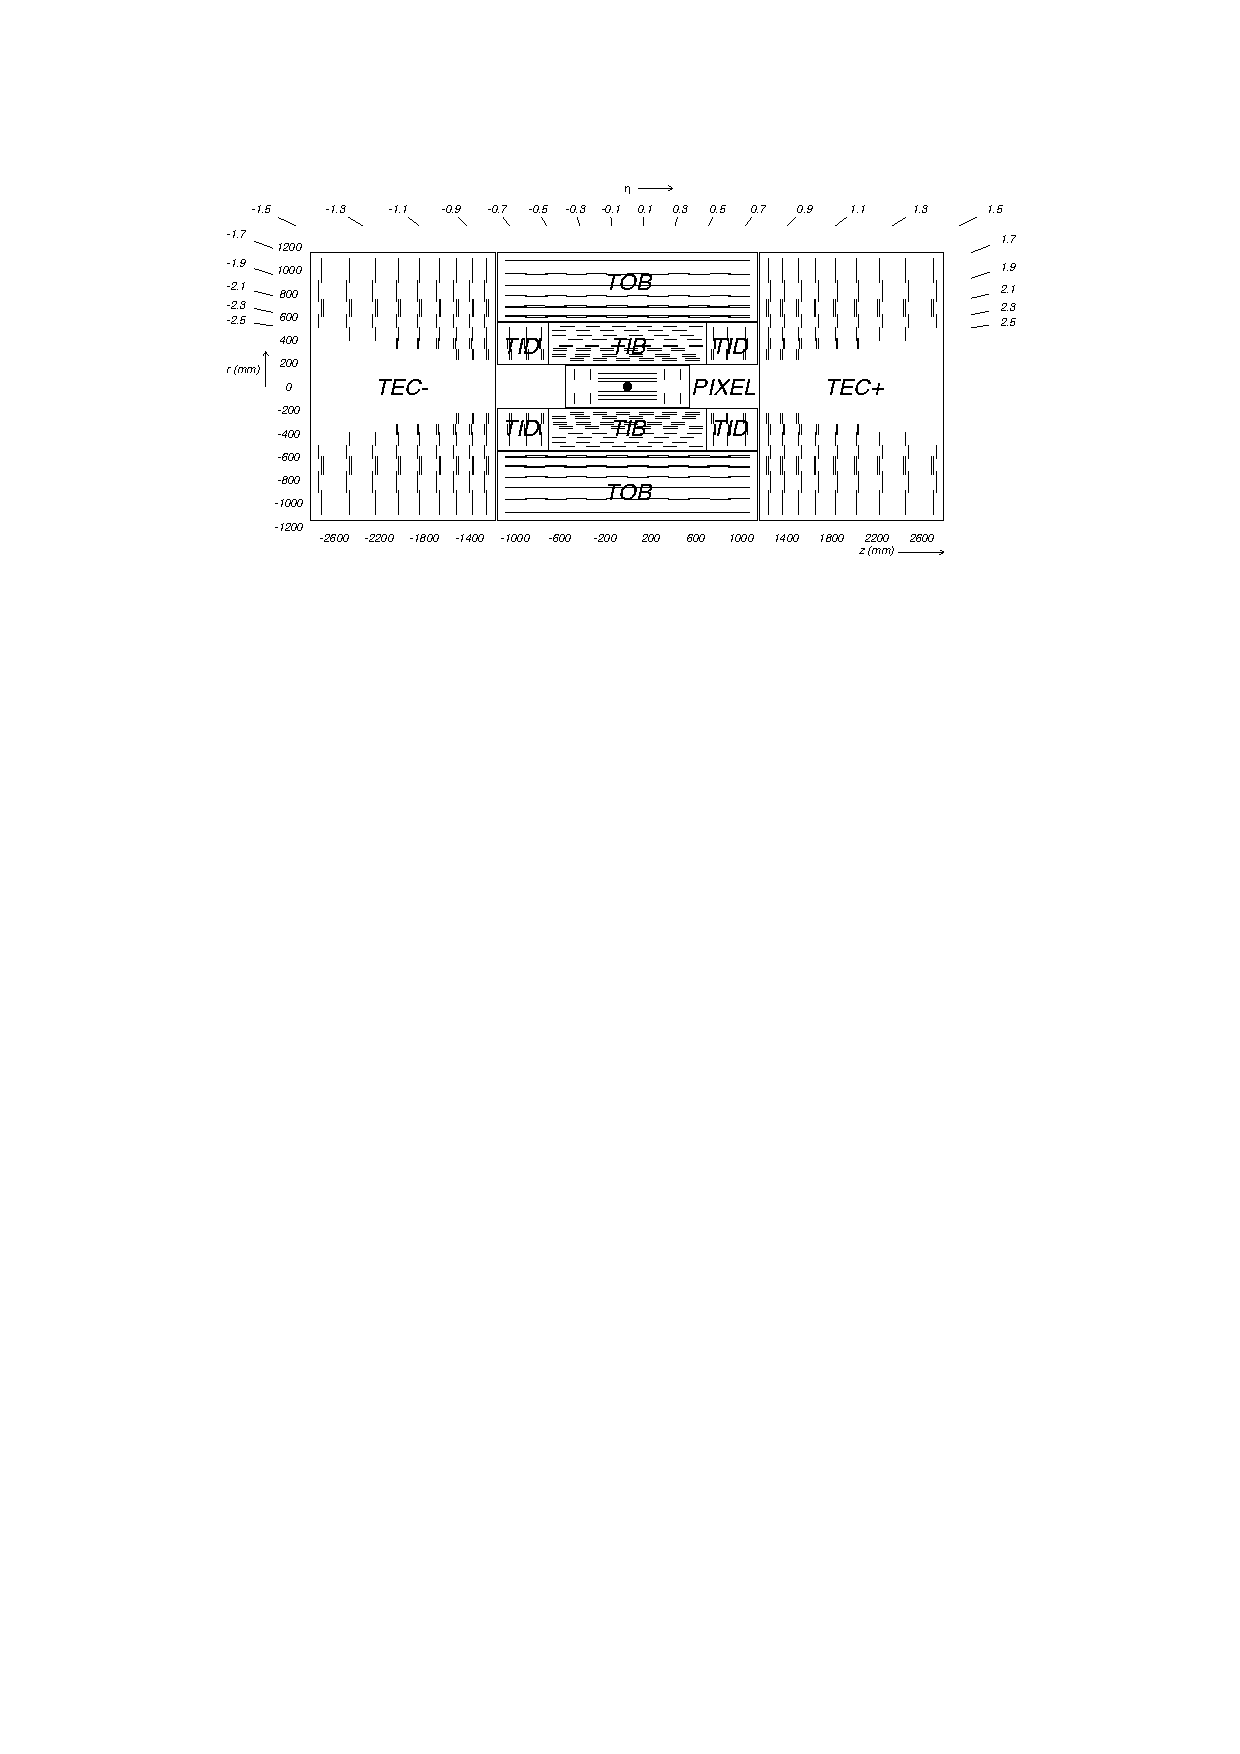
\includegraphics[width=0.6\textwidth]{figures/exp/tracker.pdf}
\caption[The CMS strip tracker]{The schematic overview of the CMS strip tracking system.}
\label{fig:cms_tracker}
\end{centering}
\end{figure}

Overall, the tracking system has to maximize the number of measurement points for each particle trajectory while keeping the material budget, measured in radiation lengths~$X_0$, at a minimum. Over the whole functional~$\eta$~range, the tracking system contributes between 0.4 and 1.8~$X_0$, with the largest radiation losses in the region around~$|\eta| \simeq 1.5$~due to the TIB/TID transition. Nevertheless, the transverse momentum resolution of muons is around~$1-2\%$~up to~$|\eta| \leq 1.6$, a reconstruction efficiency of around 99\% over most of the~$\eta$~range and of the transverse impact parameter resolution around~$10~\mathrm{\mu m}$~for high momentum tracks~\cite{Chatrchyan:2008aa}. 

The pixel detector was upgraded during the 2016-2017 winter shutdown procedure, adding an additional layer at~$r=2.9$~cm and improving the capabilities of the readout chip (ROC) to cope with an instantaneous luminosity of~$L = 2 \times 10^{34}\ \mathrm{cm}^{-2}\mathrm{s}^{-1}$~\cite{Tavolaro:2016hfj}.

\subsection{Electromagnetic calorimeter}
The primary function of the electromagnetic calorimeter is to measure the energy of electrons and photons through the production of scintillation light. The ECAL is situated within the solenoid volume in order to minimize energy losses from multiple scattering and consists of around 76000 lead-tungstenate~($\mathrm{PbWO}_4$) crystals arranged in the barrel and endcap, as seen on~\cref{fig:cms_ecal}. This material is characterized by a high density~($\rho = 8.28~\mathrm{g}/\mathrm{cm}^3$), a short radiation length ($X_0=0.89~\mathrm{cm}$) and a small Moli\`ere radius~($R_M = 2.19~\mathrm{cm}$), which characterises the transverse size of the electromagnetic shower. Furthermore, the scintillation decay time is short, such that 80\% of the light is emitted during the 25~ns bunch spacing. The light is emitted with a broad maximum in the 420-430~nm range.

In the barrel (endcaps), the crystals are coupled to avalanche photodiodes (vacuum phototriodes) for light collection, with a 1~MeV particle producing a yield of about 4.5 photoelectrons. Due to the high radiation damage expected throughout the lifetime of the ECAL, the light transmission properties of the crystals are monitored  using injected laser light at $\lambda = 440~\mathrm{nm}$. A two-layer lead absorber and silicon strip sensor preshower detector is located between the endcaps and the interaction point, covering $1.65 < |\eta| < 2.6$, in order to improve the discrimination between photons and $\pi^0$.

\begin{figure}
\begin{centering}
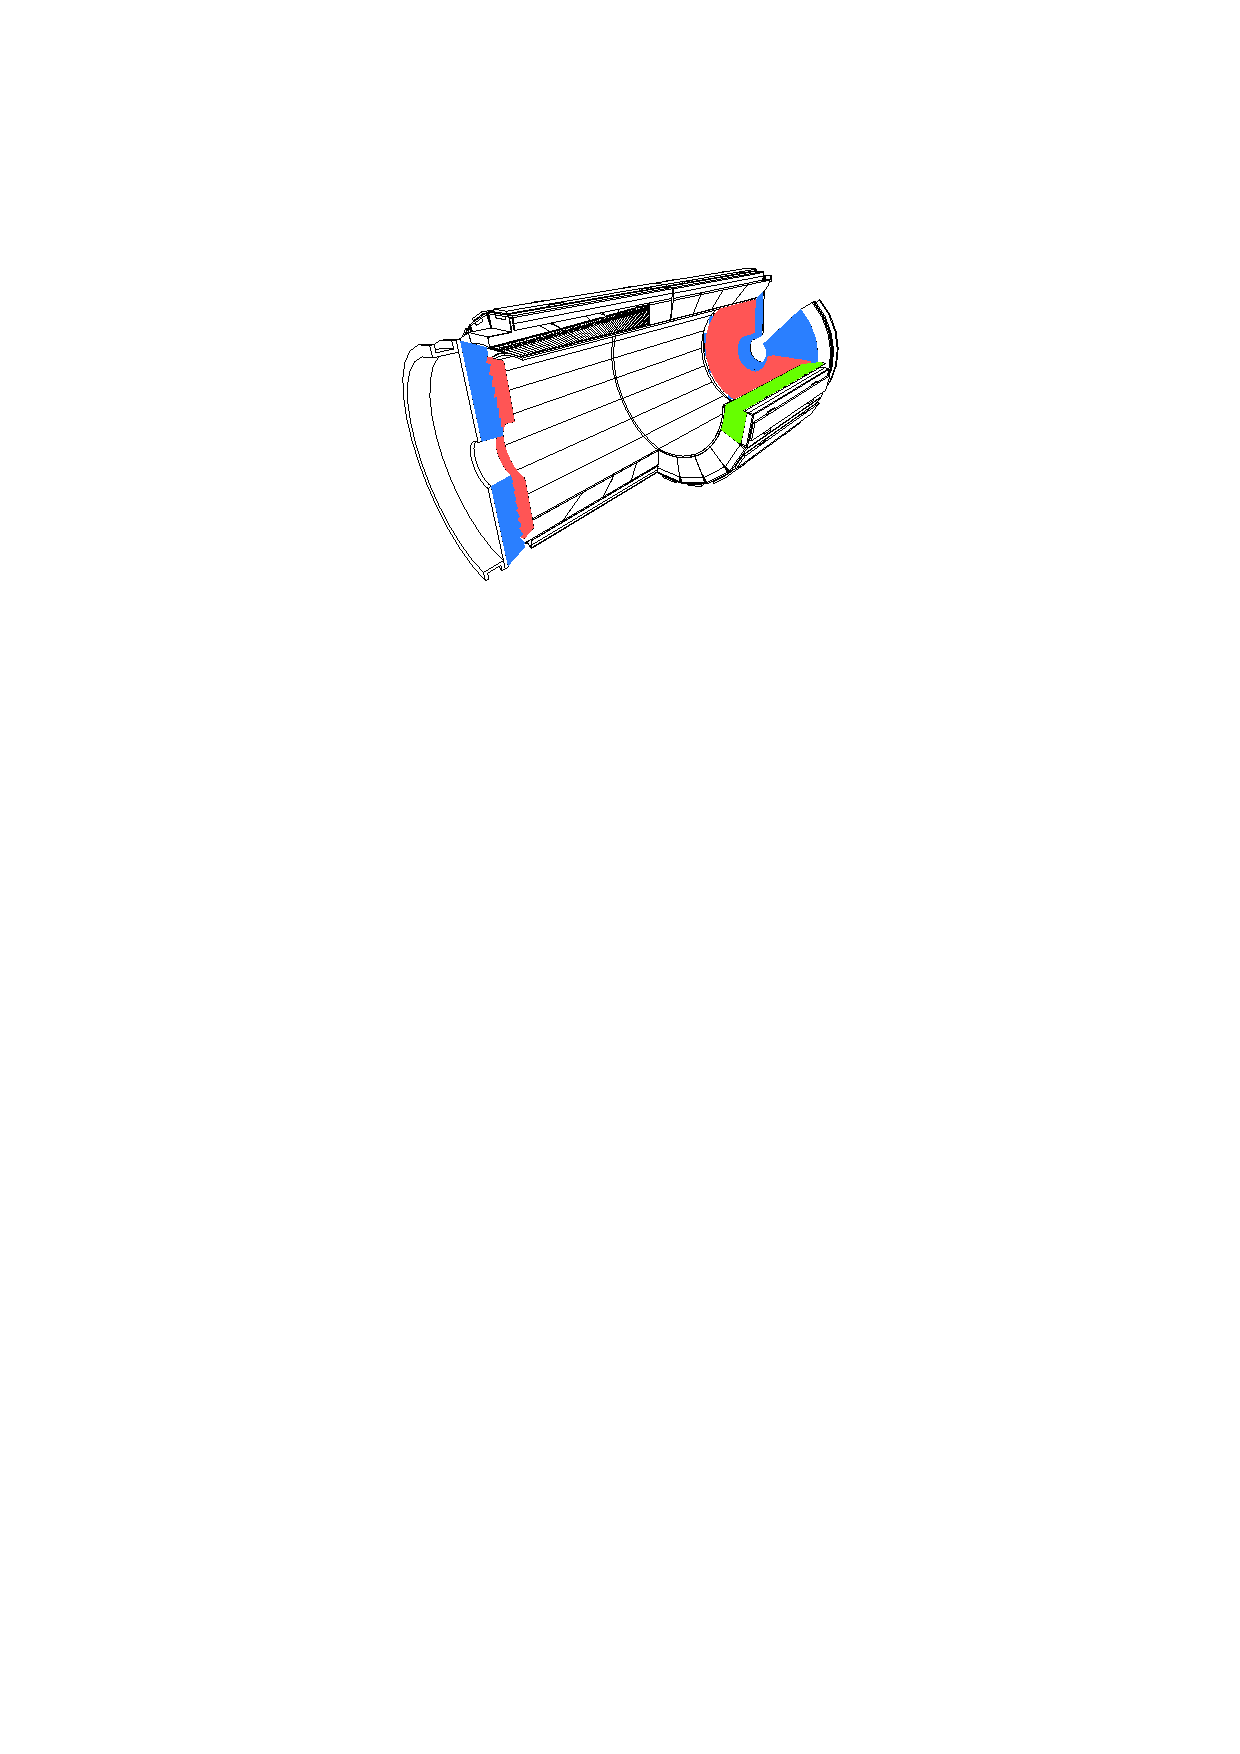
\includegraphics[width=0.6\textwidth]{figures/exp/ecal.pdf}
\caption[The structure of the CMS electromagnetic calorimeter]{The CMS electromagnetic calorimeter, with the barrel crystal clusters in green, the endcaps in blue and the preshower in red.}
\label{fig:cms_ecal}
\end{centering}
\end{figure}

The ECAL barrel region extends to~$|\eta| < 1.479$, with a 360-fold (190-fold) granularity in the azimuthal (polar) direction. The endcaps cover the range between~$1.479 < |\eta| < 3.0$. Since the photon emission in scintillation and subsequent amplification are temperature-dependent, the ECAL has to be maintained at a constant temperature within~$0.05\degree~\mathrm{C}$. In order to reconstruct the signal pulse from the photodetectors, a new technique is used in Run II, where the signal amplitude templates from up to 9 bunch crossings around the in-time signal are fitted to the observed 10-sample signal, in order to determine signal amplitude in the presence of both in-time and out-of-time pileup~\cite{Brianza:2017slq}. The energy resolution of the ECAL has been measured in electron test beams, arranging the crystals in a $3\times3$ matrix to minimize energy leakage, and found to be described by

\begin{equation}
\frac{\sigma_E}{E} = \frac{a}{\sqrt{E}} \oplus \frac{b}{E} \oplus c
\end{equation}
with $a = 2.8\%$ being the stochastic term, $b = 12\%$ the noise term and $c = 0.3\%$ the irreducible term from non-uniformities for the barrel~\cite{Adzic:2007mi}.

Since there is about $1-2X_0$ of material in front of the ECAL which results in significant multiple scattering and the crystals are about one Moliere radius in the lateral dimension, the energy from a single electromagnetic shower is spread over multiple crystals. In order to reconstruct the energy of incident particles, the energy that is spread over multiple ECAL crystals is clustered by merging crystals into superclusters. The ECAL has an excellent energy resolution, with photons from the decay of a 125-GeV Higgs boson being reconstructed in the barrel with an energy resolution between 1.1\% and 2.6\%~\cite{Chatrchyan:2013dga}.

\subsection{Hadronic calorimeter}
The purpose of the HCAL is to measure the energies of hadron jets and to have a hermetic energy coverage of the detector, such that the missing transverse energy resulting from neutrinos or hypothetical weakly interacting particles could be determined. The HCAL consists of a barrel and endcaps extending to $|\eta| < 3.0$, with a forward calorimeter covering the range up to $|\eta|<5.0$, as seen on~\cref{fig:hcal}.

\begin{figure}
\begin{centering}
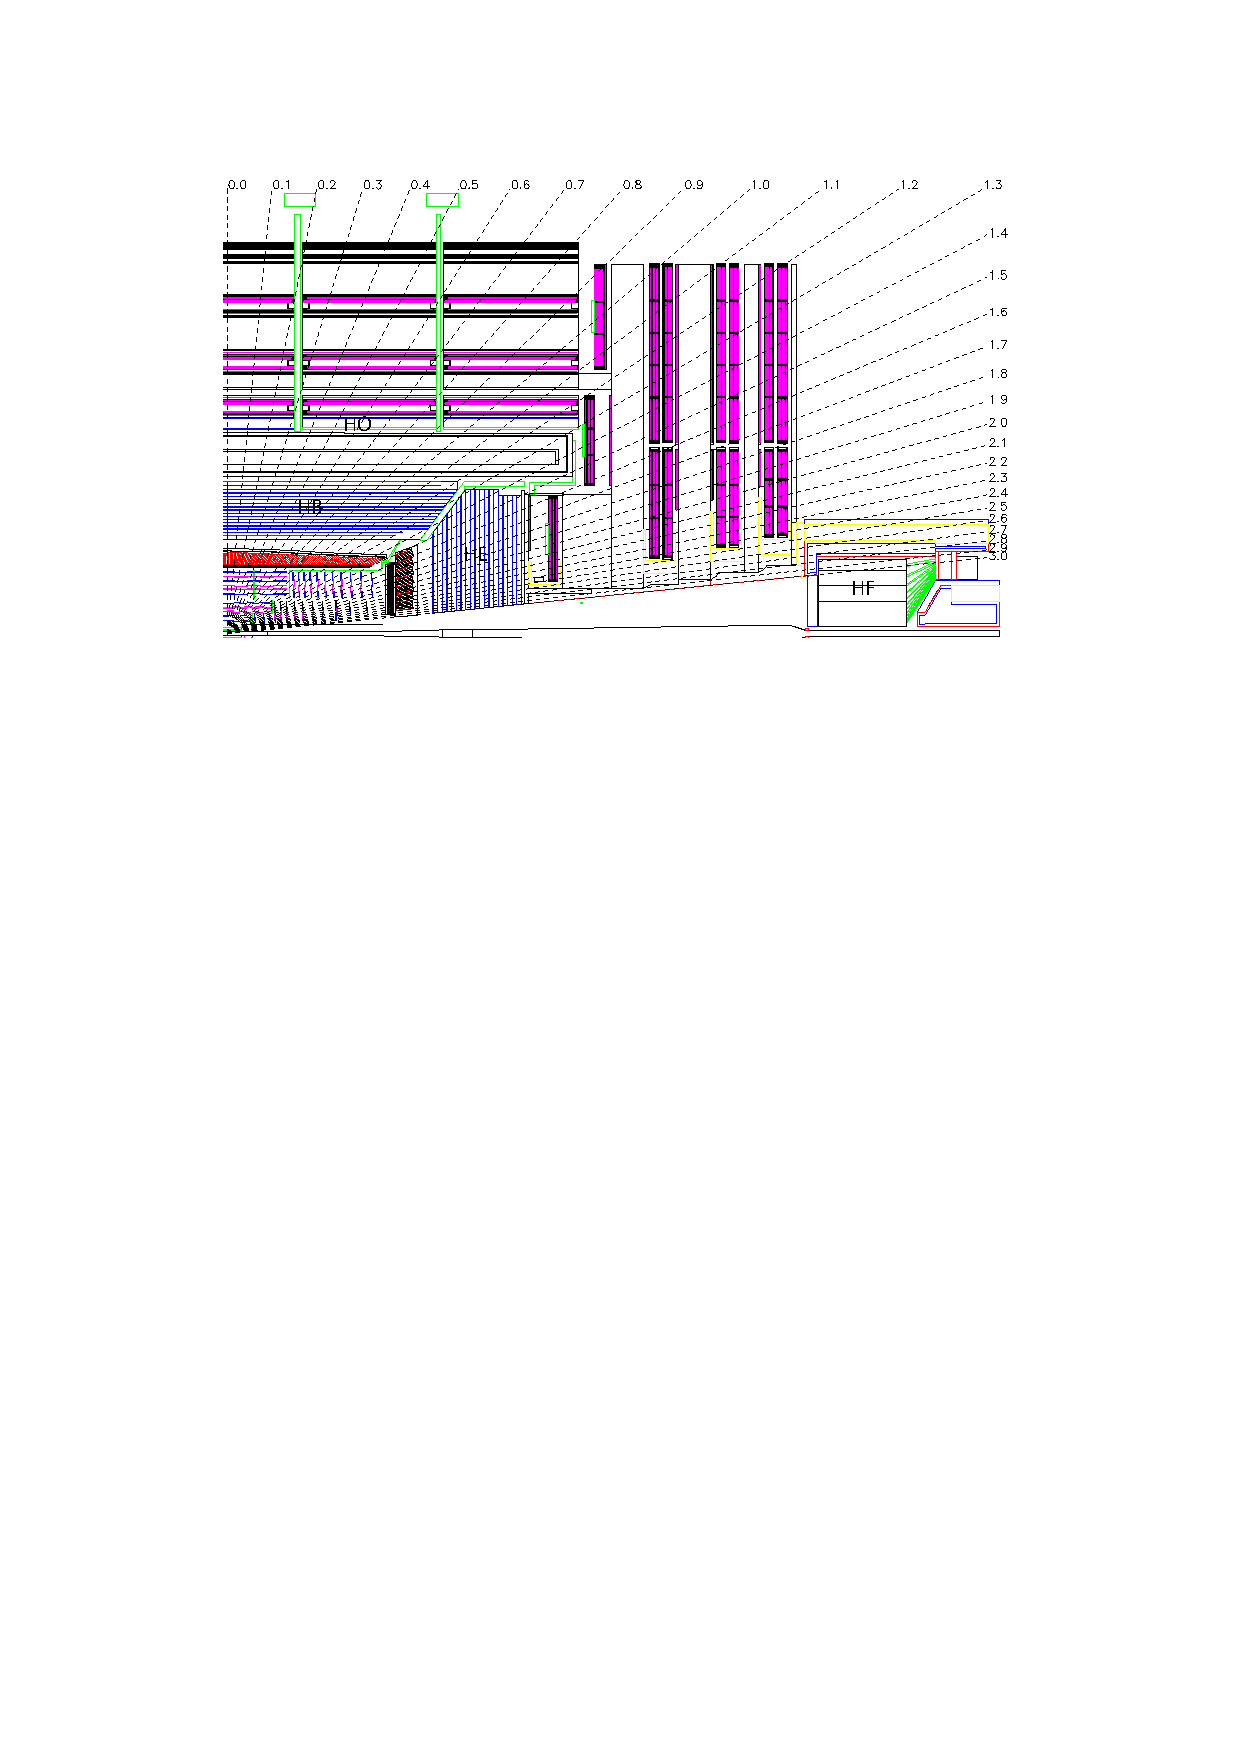
\includegraphics[width=0.6\textwidth]{figures/exp/hcal.pdf}
\caption[The cross-section of the CMS hadronic calorimeter]{The cross-section of the CMS hadronic calorimeter, showing the barrel region (HB), the endcap (HB), the outer calorimeter (HO) and the forward calorimeter (HF).}
\label{fig:hcal}
\end{centering}
\end{figure}


The HCAL barrel is situated between the ECAL and the superconducting coil in the region~$1.77~\mathrm{m} < R < 2.95~\mathrm{m}$. As this limits the amount of material, an outer hadron calorimeter is installed outside the solenoid in the barrel region, such that the material amounts to around 11 hadronic radiation lengths. The HCAL barrel regions extends to $|\eta| < 1.3$ and consists of an absorber made from brass sandwiched between steel plates with embedded scintillator tiles. The scintillation light is read out by bringing the light to photodiodes in readout towers using wavelength shifting fibres. Hybrid photodiodes are used due to their low sensitivity to the magnetic field and their large dynamical range.

The HCAL endcaps cover the pseudorapidity range $1.3 < |\eta| < 3$, thus they need to handle high counting rates and be radiation hard. They follow a similar construction as the barrel, with an absorber/scintillator design with a segmentation granularity of~$\Delta \eta \times \Delta \phi = 0.087 \times 0.087$~for~$|\eta| < 1.6$~and~$\Delta \eta \times \Delta \phi \simeq 0.17 \times 0.17$ for the rest of the endcap.

The forward calorimeter (HF) located at $\pm$11 m from the interaction point, covering the range $3.0 < |\eta| < 5.2$, is situated in an extreme radiation environment of up to 100 Mrad/year, thus radiation hardness has been the primary design criterion. It is based on the collection of Cherenkov light collected in quartz fibres embedded in steel absorber plates, read out by photomultiplier tubes. The HF is mostly sensitive to the electromagnetic component of showers~\cite{Akchurin:2003tp}. The HF can be used for luminosity monitoring in CMS to infer the mean number of interactions per bunch crossing and thus an accurate determination of the normalization for physics analyses.

The energy resolution of the HCAL has been determined in test beams using single pions and found to be approximately~$\sigma/E = 110\%/\sqrt{E} \oplus 9\%$~\cite{Elvira:2004iya} with a typical readout noise of 200~MeV per tower. The particle flow algorithm is further used to build a global representation of the event based on the detector signals from other subsystems~\cite{CMS-PRF-14-001}.

\subsection{The muon systems}
Muon detection is of central importance to CMS, as they can be detected relatively easily and are produced in several interesting decays, such at $\mathrm{H} \rightarrow \mathrm{Z} \mathrm{Z}^* \rightarrow 4 \mathrm{\mu}$. The muon systems in CMS are used to identify muons over a wide angular range up to $|\eta| < 2.4$, to measure their charge and momentum and for triggering purposes. The punch-through of other particles to the muon systems is negligible due to the amount of material, which is around 16$X_0$. The muon reconstruction efficiency is around 95-99\% and the $p_T$-resolution between 15\% in the barrel and 25\% in the endcap, which is necessary to use the muon system for triggering. Since the muon systems cover a large area around the detector in the form of a barrel and endcaps, they have to be inexpensive and robust.

In the barrel region, drift tubes that are organized into 4 stations arranged in concentric cylinders within the return yoke. The drift tubes use a mixture of~$\mathrm{Ar}/\mathrm{CO}_2$~gas and each chamber consists of 4 layers arranged into a superlayer. This provides a timing resolution of a few nanoseconds and allows the muon system readout to be assigned to a bunch crossing. The spatial resolution of the drift chambers has been measured in test beams to be around~$300~\mathrm{\mu m}$, determined by the dispersion of the drift time and distortions of the drift caused by magnetic fields. The bunch crossing identification efficiency, which is important for triggering, is better than 90\%, driven by the timing resolution and muons producing electromagnetic showers.

In the endcaps, the muon system consists of cathode strip chambers (CSC), which have the advantage that they can operate at the high rates and non-uniform magnetic field present in the forward region. The spatial resolution of a hit is around~$\sim 80~\mathrm{\mu m}$~in the combined 6-plane CSC chamber and the bunch tagging efficiency is around 98-99\%.

In order to complement the time resolution of the drift tubes and the CSC, a trigger system based on resistive place chambers (RPC) exists in the barrel and endcaps. The RPC operates on the principle of an avalanche generated in a gas gap between two resin plates, such that the bunch crossing assignment can be done with rates up to~$1~\mathrm{kHz}/\mathrm{cm}^2$. The timing resolution of a few nanoseconds provided by the RPC crucially improves the trigger efficiency.

Since manufacturing tolerances, the intense magnetic field and thermal stress can cause the geometry of the muon system to change at the level of up to a few centimeters, it is monitored using an optical alignment system~\cite{Chatrchyan:2009sr}. 

\subsection{Trigger, data acquisition and computing}
The data from the 40~MHz LHC collisions needs to be reduced by a factor of $10^6$ for storage and analysis. This means that some form of triggering needs to be applied in order to select the most interesting physics events containing high-energy particles. The CMS experiment employs a 2-level trigger system, where the Level-1 (L1) trigger is implemented in custom programmable electronics and operates on the level of the calorimeters and the muon systems, whereas the high-level trigger (HLT) has access to the complete event read-out and is implemented on a conventional CPU farm.

The L1 trigger is composed of the trigger primitive generators, which operate on the level of calorimeter trigger towers, track segments and hit patterns on muon chambers.  This information is combined using regional triggers to determine trigger objects in limited spatial regions of the detector. These objects are then compared by the global calorimeter and muon triggers, which determine if sufficient good-quality muon or calorimeter objects are present to accept the event. The processing is pipelined such that the deadtime is minimized.

The global calorimeter trigger works on the basis of jets, total transverse energy, missing transverse energy and $H_T$, the scalar transverse energy sum of jets. Furthermore, it provides isolated and non-isolated $\mathrm{e}/\mathrm{\gamma}$ candidates. The muon system trigger works on the basis of reconstructing track candidates from hits in the drift tubes, the CSCs and the RPCs. In the global muon trigger, the muon candidates are identified by $p_T$, charge, $\eta$, $\phi$ and quality parameters, as well as isolation information from the global calorimeter trigger primitive.

The data with a maximal output rate of 100~kHz from the L1 trigger is fed into the HLT, which further reduces the recorded events to a rate of about 100~Hz. The data are divided to luminosity sections of~$2^{20}$~LHC orbits~(93~s), during which trigger thresholds and trigger prescale factors, which sample the trigger acceptance, are not changed. The total amount of zero-suppressed data recorded for a bunch crossing is on the order of 1~MB.

If an event is accepted by the HLT, it is transferred to the CMS offline computing infrastructure, which consists of several computing tiers with the bulk of the computing resource located in computing centres around the globe. The Tier 0 center at CERN performs the prompt reconstruction of the data and transfers it to several Tier 1 centres for storage, where late-stage reconstruction with improved calibrations can take place. Data analysis and MC simulation happens primarily at Tier 2 centres, which are associated to Tier 1 sites and divide the resources between the CMS collaboration and the local physics community. A typical Tier 2 site hosts 1-2~PB of data and O(5000) CPUs.

\subsection{Particle flow reconstruction}
\label{sec:particleflow}
In case collision event passes the HLT, it is recorded as signals from different subsystems of the detector, such as calorimeter deposits and muon system hits. In CMS, the reconstruction algorithm creates physics objects such as jets, leptons and missing transverse energy by linking the signals across different sub-detectors using the particle flow (PF) algorithm to arrive at a global event description. This algorithm relies on high-granularity sub-detectors, which allow signals from various subsystems to be correlated. 

The PF algorithm associates tracks to calorimeter clusters based on geometrical proximity and at a qualitative level proceeds by ``subtracting'' objects from the event in order of decreasing reconstruction accuracy, starting from muons, followed by electrons and isolated photons, such that neutral hadrons and non-isolated photons are built from calorimeter clusters that are not associated to any tracks. The PF algorithm improves the resolution of the detector, with the jet response $R = p_T / p_{T,\mathrm{ref}}$ measured with respect to the particle-level reference jet is corrected from around 60\% at $p_T = 100~\mathrm{GeV}$ to around $R=95\%$, significantly reducing the momentum dependence~\cite{cms_particleflow:2017}.

\section{Summary}
Overall, the LHC is uniquely suited to studying the Higgs boson and thus the mechanism of electroweak symmetry breaking in high-energy processes. The accelerator has been operating close to design capabilities with around $35-40~\mathrm{fb}^{-1}$ of integrated luminosity in proton-proton collisions delivered per year at the centre-of-mass energy of 13 TeV. The CMS experiment has excellent characteristics for detecting and studying the SM particles produced in the~\ttH~process and in the subsequent decay, thus making it possible to experimentally clarify the nature of the recently-discovered Higgs boson by determining the coupling of the scalar field to fermions.

